\documentclass[12pt]{article}

\usepackage[T1]{fontenc}
\usepackage[utf8]{inputenc}

\usepackage{amsmath,amssymb,mathtools}
\usepackage{geometry}
\usepackage{float}
\usepackage{placeins}
\usepackage{hyperref}

\geometry{margin=2.5cm}

\setlength{\parindent}{0pt}
\setlength{\parskip}{4pt}

\newcommand{\dd}{\mathrm{d}}
\newcommand{\pd}[2]{\frac{\partial #1}{\partial #2}}
\newcommand{\pdd}[2]{\frac{\partial^2 #1}{\partial #2^2}}

\title{A Concise End-to-End Strategy Overview}
\author{Egor Shiryaev}
\date{}

\begin{document}

\maketitle

\noindent Jupyter notebook: \href{https://github.com/tenzenmonsta/End-to-end-quant-strategy}{End-to-end GH}

\section{Trading Hypothesis and Motivation}
\textbf{Hypothesis:} liquid Russian equities exhibit persistent medium-term trends.
Combining \textit{trend-following} and \textit{volatility targeting} improves the portfolio's risk profile relative to passive buy-and-hold.

\medskip
\textbf{Expected effect:}
\begin{itemize}
    \item participation in directional market moves;
    \item reduced risk during periods of high volatility;
\end{itemize}

\subsection*{Economic Rationale}
\begin{itemize}
    \item \textbf{Momentum:} assets with positive recent performance often continue to trend.
    \item \textbf{Volatility clustering:} sizing the position via a \textit{target vol} rule stabilizes risk.
\end{itemize}

\subsection*{Implementation Idea}
The strategy uses a trend filter and volatility-target position scaling to achieve a more stable risk-adjusted return relative to a passive equal-weighted portfolio.


\subsection*{Criteria for Production Readiness}

\begin{enumerate}
    \item \textbf{Out-of-sample robustness}
    \begin{itemize}
        \item stable results across walk-forward periods;
        \item a controlled level of drawdowns.
    \end{itemize}

    \item \textbf{Robustness to costs}
    \begin{itemize}
        \item the strategy remains viable under realistic commissions and spreads;
    \end{itemize}

    \item \textbf{Parameter robustness}
    \begin{itemize}
        \item small changes in \textit{lookback} / \textit{vol-target} should not break the strategy;
    \end{itemize}

    \item \textbf{Risk control}
    \begin{itemize}
        \item bounded \textit{max drawdown};
        \item stable portfolio volatility;
    \end{itemize}

    \item \textbf{Practical feasibility}
    \begin{itemize}
        \item liquid instruments are used;
        \item a reasonable rebalancing frequency.
    \end{itemize}
\end{enumerate}
\section{Data Acquisition and Retrieval}

Data was loaded via T-Bank's \textit{Tinkoff Invest API}: historical candles for each instrument, and dividends.

The project used both synchronous and asynchronous loading modes. The asynchronous path speeds up data collection across multiple instruments: while one request is waiting for a response from the API, the program can issue other requests.

\section{Price Data Processing}

After receiving data from the broker, the price series must be brought into a uniform, backtest-ready form. In this project, processing consisted of two main steps:
\begin{itemize}
    \item handling gaps in the price series;
    \item adjusting prices for dividends.
\end{itemize}

\subsection*{Handling Gaps}

Gaps were handled using the \texttt{ffill().dropna()} scheme:
\begin{itemize}
    \item \texttt{ffill()} --- fills gaps with the last available price;
\end{itemize}

\texttt{ffill()} was chosen because it uses only information available at the time of observation and does not leak data from the future. This matters for a correct backtest and for computing trading signals.

The \texttt{bfill()} approach (filling with a future value) was not used, since it can introduce \textit{look-ahead bias}. For the same reason, the \texttt{ffill().bfill()} scheme was not applied: although it formally removes more gaps, it can fill values with future prices and make the backtest results methodologically invalid.

\subsection*{Dividend Price Adjustment}

An additive dividend price adjustment was used to correctly compute price returns. Without this adjustment, ex-dividend dates create downward jumps in the price series that are unrelated to market movement and can distort returns, volatility, and trading signals.

\subsubsection*{Adjustment Concept}
Let $P_t$ be the price at time $t$, $D_u$ the per-share dividend paid at time $u$, and $P_t^{adj}$ the adjusted price. The additive adjustment is then given by
\[
P_t^{adj} = P_t - \sum_{u>t} D_u.
\]

In other words, the sum of all future dividends is subtracted from the historical price to remove the effect of ex-dividend dates from the price series.

\subsubsection*{Implementation Details}
The implementation used per-instrument dividend data, with future payouts accumulated along the timeline. Stock splits were also accounted for: dividends paid before a split date were rescaled by the split ratio so the adjustment stays consistent with the current price scale.

\subsubsection*{A Note on Validation}
If desired, the adjustment can be cross-checked against external sources (e.g., \textit{yfinance}), but the absolute levels of adjusted prices may differ due to differences in how dividends and corporate actions are handled. It is therefore more appropriate to compare derived quantities, chiefly returns (\texttt{pct\_change()}), rather than price levels.

\section{Building the Benchmark: an Equal-Weighted Portfolio}

The benchmark was a passive equal-weighted portfolio of the selected liquid stocks. This benchmark lets us compare the strategy's results not against a single instrument, but against a diversified buy-and-hold alternative on the same set of names.

\subsection*{Construction Principle}
On each rebalancing date, capital is split equally across all assets. If the portfolio holds $N$ instruments, each instrument's weight is
\[
w_i = \frac{1}{N}, \qquad i = 1, \dots, N.
\]
\begin{figure}[h!]
    \centering
    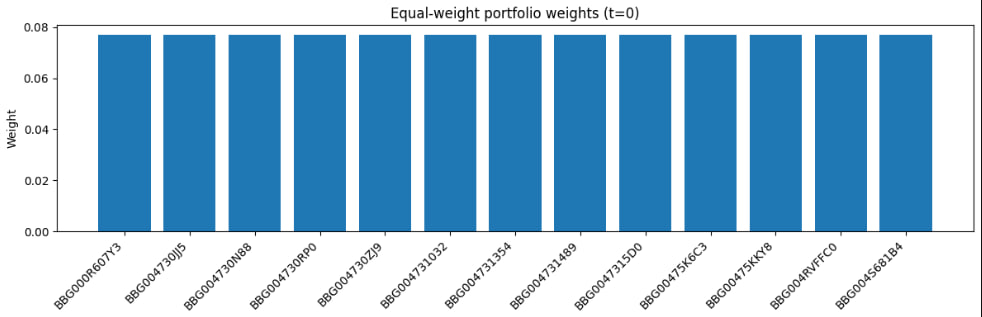
\includegraphics[width=\linewidth]{equal_portfolio}
    \caption{Initial weights of the equal-weighted benchmark portfolio.}
    \label{fig:benchmark_weights}
\end{figure}

\subsection*{Preliminary Analysis of the Benchmark Portfolio}

After building the benchmark portfolio, a basic diagnostic analysis of its properties was carried out to establish a reference point for comparison with the strategy.

\textbf{Distribution of Daily Returns.}
The histogram of the benchmark portfolio's daily returns lets us assess the shape of the distribution, any skew, and the tail behavior.

\begin{figure}[H]
    \centering
    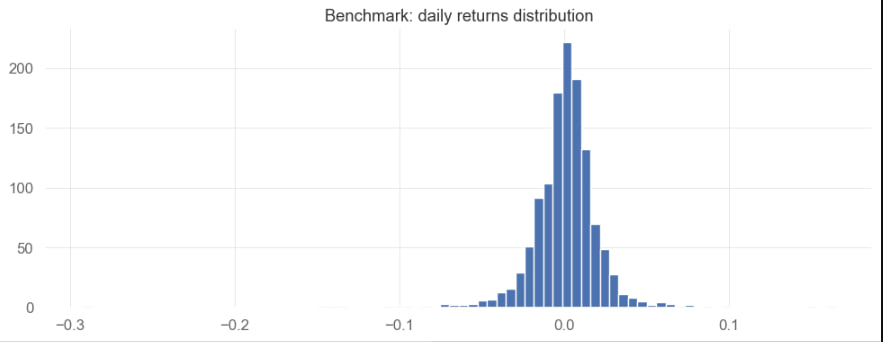
\includegraphics[width=0.82\linewidth]{benchmark_returns_distribution}
    \caption{Distribution of the benchmark portfolio's daily returns.}
    \label{fig:benchmark_returns_distribution}
\end{figure}

\textbf{QQ-Plot of Daily Returns.}
The QQ-plot is used to visually check for deviations of the return distribution from normality.

\begin{figure}[H]
    \centering
    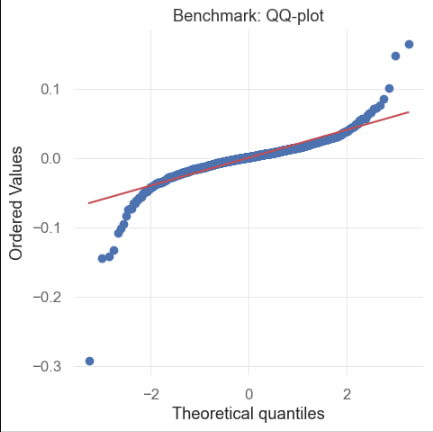
\includegraphics[width=0.55\linewidth]{benchmark_qqplot}
    \caption{QQ-plot of the benchmark portfolio's daily returns.}
    \label{fig:benchmark_qqplot}
\end{figure}

Based on this preliminary diagnostic, we can assess the shape of the return distribution and possible deviations from normality.

\FloatBarrier
\clearpage

\textbf{Correlation Structure of the Assets.}
The correlation matrix shows the degree of co-movement between the stocks and lets us assess the benchmark portfolio's actual diversification.

\begin{figure}[H]
    \centering
    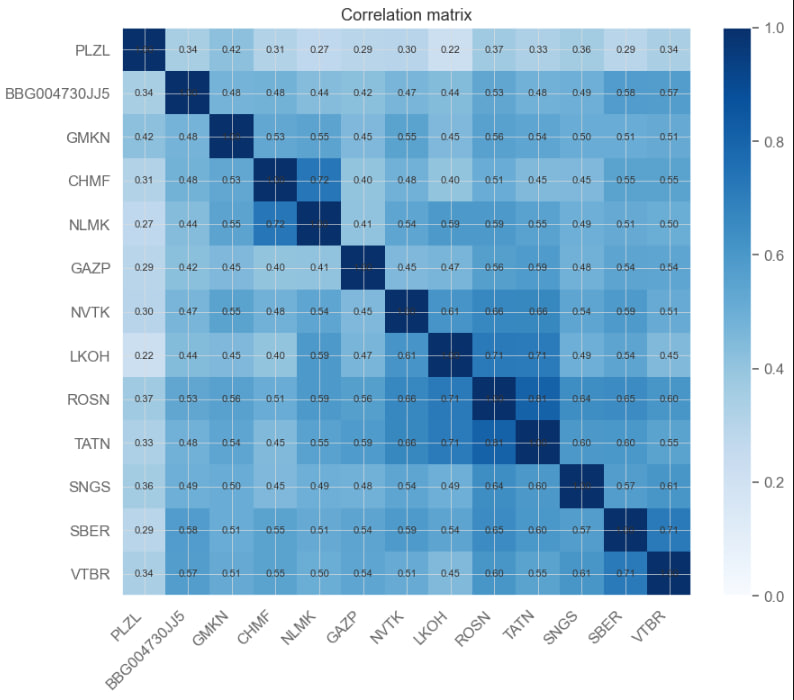
\includegraphics[width=0.88\linewidth]{benchmark_corr_matrix}
    \caption{Correlation matrix of the benchmark portfolio's asset returns.}
    \label{fig:benchmark_corr_matrix}
\end{figure}


\FloatBarrier

\section{Trading Strategy: Trend Filter and Volatility Targeting}

The strategy is built as an overlay on top of the benchmark portfolio (the equal-weighted stock portfolio). Rather than picking individual names, the strategy manages exposure to the benchmark: it increases or decreases the fraction of capital held in the base portfolio depending on the market regime and current volatility.

\subsection*{Core Idea}
Two simple, interpretable rules are used:
\begin{itemize}
    \item \textbf{trend filter:} risk is held only when the benchmark's equity curve is above its moving average;
    \item \textbf{volatility targeting:} position size is scaled to maintain the strategy's target volatility level.
\end{itemize}

The strategy thus combines filtering out unfavorable market regimes with risk control via dynamic exposure management.

\subsection*{Formalization}
Let \(r_t^{(b)}\) be the benchmark portfolio's return, and \(x_t\) the strategy's exposure to the benchmark.

\textbf{1) Trend filter.}
The benchmark returns are used to build an equity curve:
\[
E_t = \prod_{u \le t}(1+r_u^{(b)}).
\]
If \(E_t\) is above its moving average, risk is ``on''; otherwise exposure is reduced.

\textbf{2) Volatility targeting.}
The realized volatility estimate \(\widehat{\sigma}_t\) is computed over a rolling window. The target exposure is given by
\[
x_t \propto \frac{\sigma^\star}{\widehat{\sigma}_t},
\]
where \(\sigma^\star\) is the target annualized volatility. In practice, exposure is capped from above (a leverage cap).

\textbf{3) Strategy return.}
For a correct backtest, the lagged exposure \(x_{t-1}\) is used (no look-ahead bias). The strategy's return then combines the benchmark return and the cash return:
\[
r_t^{(\text{strat})} = x_{t-1} r_t^{(b)} + (1-x_{t-1}) r_t^{(cash)} - c_t,
\]
where \(c_t\) is the rebalancing cost, proportional to the change in exposure.

\subsection*{Diagnostics of Strategy Returns}

As a first diagnostic of the strategy's results, we examine the distribution of daily returns. The histogram lets us visually assess the concentration of observations near zero, the skew, and the tail behavior.

\begin{figure}[H]
    \centering
    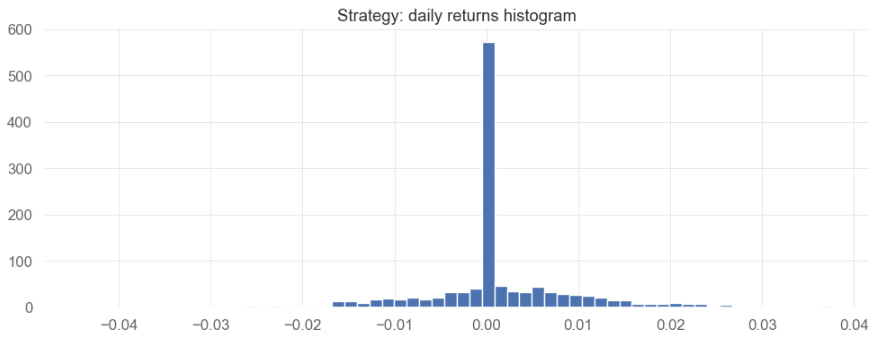
\includegraphics[width=0.82\linewidth]{strategy_returns_hist}
    \caption{Histogram of the strategy's daily returns.}
    \label{fig:strategy_returns_hist}
\end{figure}

The high concentration of values near zero reflects periods of reduced or zero exposure to the benchmark portfolio (for example, when the trend filter is off), as well as the effect of exposure smoothing and the cash component.
\subsection*{6. Walk-Forward Validation with an Embargo}

To assess the robustness of the results, we used walk-forward out-of-sample validation over the time series, with an embargo gap between the training and test windows.

At each step, a historical window (\(L_{\text{back}}\)) was formed, followed by an embargo gap (\(L_{\text{emb}}\)), after which performance was evaluated on the subsequent test interval (\(L_{\text{fwd}}\)). The window was then shifted forward and the procedure repeated.

The embargo is introduced to reduce information leakage between adjacent windows and to lower spurious correlation between out-of-sample metrics at neighboring validation steps.

\begin{figure}[H]
    \centering
    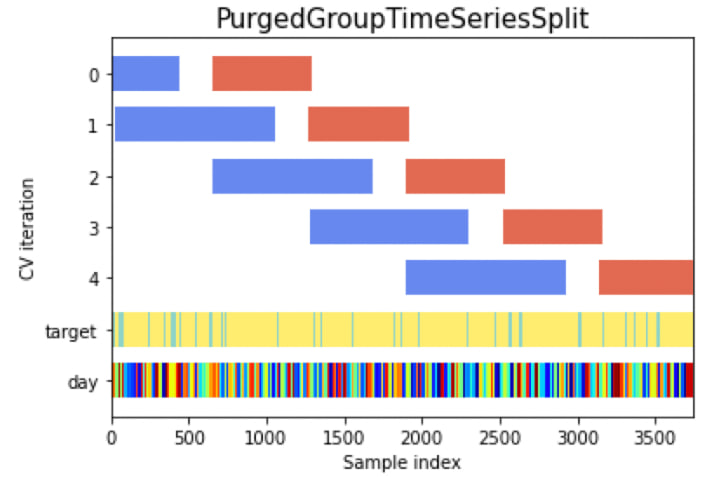
\includegraphics[width=0.62\linewidth]{walkforward_embargo_scheme}
    \caption{Diagram of walk-forward validation with an embargo gap.}
    \label{fig:walkforward_embargo_scheme}
\end{figure}

\subsection*{Computing Out-of-Sample Metrics}

After running the walk-forward validation, key performance metrics were computed for each out-of-sample window: \textit{Total Return}, \textit{Annualized Return}, \textit{Annualized Volatility}, \textit{CVaR}, \textit{Sharpe Ratio}, and \textit{Drawdown}. This lets us look not only at the average result but also at the spread of metrics across different market regimes.

For the final diagnostic, the distribution of these metrics was plotted across all OOS windows, giving a more robust picture of the benchmark portfolio's behavior over time.

\begin{figure}[H]
    \centering
    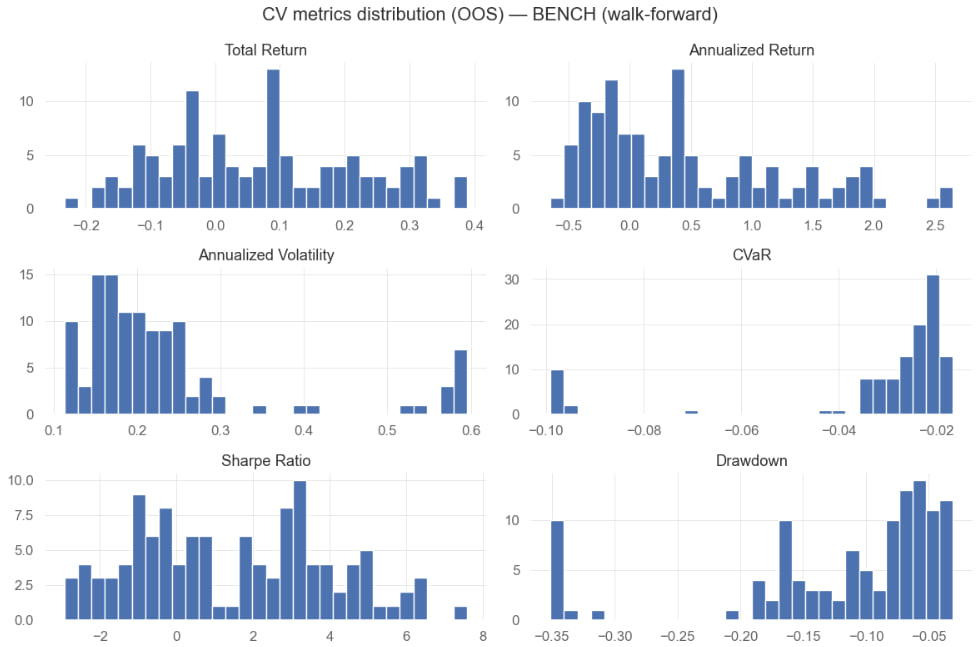
\includegraphics[width=0.92\linewidth]{metrics}
    \caption{Distribution of out-of-sample metrics}
    \label{fig:oos_metrics_distribution_bench}
\end{figure}

\subsection*{7. Backtest Results: PnL, Equity, and Comparison with the Benchmark}

Once the strategy's rules were specified (trend filter, volatility targeting, cash component, and costs), a backtest was run on the historical return series of the benchmark portfolio. From the backtest, the strategy's daily returns \(r_t^{(\text{strat})}\) were computed, from which the equity curve and cumulative PnL were built.

The following views were used to interpret the results:
\begin{itemize}
    \item the strategy's cumulative PnL;
    \item the benchmark portfolio's cumulative PnL (\textit{buy-and-hold}), for comparison;
    \item cumulative rebalancing costs;
    \item the strategy's equity curve (\textit{Market Value});
    \item intra-month PnL reset to zero at the start of each month (\textit{monthly-reset PnL}).
\end{itemize}

The \textit{monthly-reset PnL} chart is used as a more readable view of the strategy's local dynamics: it lets us visually assess intra-month moves, drawdowns, and recoveries without the compounding effect of a long horizon.

\begin{figure}[H]
    \centering
    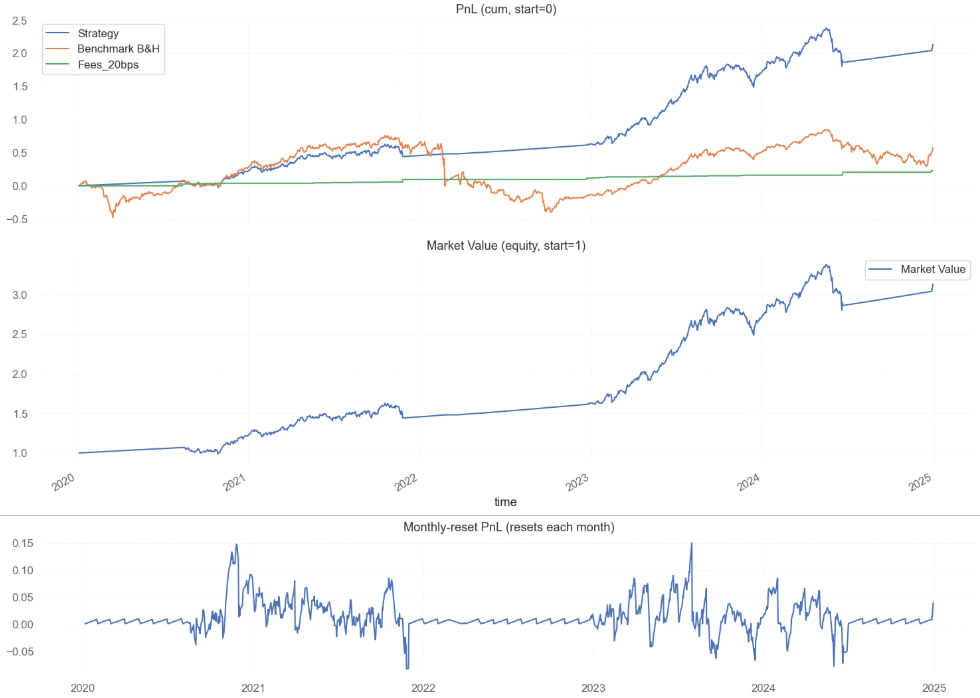
\includegraphics[width=0.95\linewidth]{results}
    \caption{Strategy backtest results: cumulative PnL, equity curve, and monthly-reset PnL.}
    \label{fig:backtest_results}
\end{figure}

\subsection*{8. Final Results, Metric Comparison, and Conclusions}

In the final step, the key metrics of the strategy and the benchmark portfolio were computed and compared (using, among other things, the \textit{quantstats} library): return, volatility, Sharpe ratio, drawdown, and return-distribution characteristics. This comparison lets us assess not just the absolute result, but the quality of the strategy's risk relative to the passive approach.

\textbf{Conclusion on the Trading Hypothesis.}
This study tested the hypothesis that combining trend-following with volatility targeting can improve the risk profile of a portfolio of liquid Russian equities relative to passive buy-and-hold.

The backtest and walk-forward analysis results show that the strategy:
\begin{itemize}
    \item exhibits a more stable return distribution;
    \item has a controlled level of drawdowns;
    \item is sensitive to transaction costs, but remains robust within reasonable ranges;
    \item remains effective on out-of-sample periods.
\end{itemize}

Using volatility targeting stabilizes the portfolio's risk, while trend filtering reduces participation in unfavorable market regimes.

As a result, the strategy can be considered a candidate for further testing in \textit{paper trading} mode and subsequent production use, subject to risk limits and regular metric monitoring.

\end{document}
